\documentclass[12pt]{article}

\usepackage{tikz} % картинки в tikz
\usepackage{microtype} % свешивание пунктуации
\usepackage{array} % для столбцов фиксированной ширины
\usepackage{comment} % для комментирования целых окружений
\usepackage{indentfirst} % отступ в первом параграфе

\usepackage{sectsty} % для центрирования названий частей
\allsectionsfont{\centering}

\usepackage{amsmath, amssymb, amsthm, amsfonts} % куча стандартных математических плюшек

\usepackage[top=2cm, left=1cm, right=1cm, bottom=2cm]{geometry} % размер текста на странице
\usepackage{lastpage} % чтобы узнать номер последней страницы
 
\usepackage{enumitem} % дополнительные плюшки для списков
%  например \begin{enumerate}[resume] позволяет продолжить нумерацию в новом списке

\usepackage{caption} % подписи к рисункам
\usepackage{hyperref} % гиперссылки
\usepackage{multicol} % текст в несколько столбцов


\usepackage{fancyhdr} % весёлые колонтитулы
\pagestyle{fancy}
\lhead{Введение в глубокое обучение, ЭМИТ, РАНХ}
\chead{}
\rhead{2022-04-27}
\lfoot{Вариант $da$}
\cfoot{Паниковать запрещается!}
%\rfoot{Тест}
\renewcommand{\headrulewidth}{0.4pt}
\renewcommand{\footrulewidth}{0.4pt}

\usepackage{ifthen} % для написания условий

\usepackage{todonotes} % для вставки в документ заметок о том, что осталось сделать
% \todo{Здесь надо коэффициенты исправить}
% \missingfigure{Здесь будет Последний день Помпеи}
% \listoftodos --- печатает все поставленные \todo'шки


% более красивые таблицы
\usepackage{booktabs}
% заповеди из докупентации:
% 1. Не используйте вертикальные линни
% 2. Не используйте двойные линии
% 3. Единицы измерения - в шапку таблицы
% 4. Не сокращайте .1 вместо 0.1
% 5. Повторяющееся значение повторяйте, а не говорите "то же"


\usepackage{fontspec}
\usepackage{polyglossia}

\setmainlanguage{russian}
\setotherlanguages{english}

% download "Linux Libertine" fonts:
% http://www.linuxlibertine.org/index.php?id=91&L=1
\setmainfont{Linux Libertine O} % or Helvetica, Arial, Cambria
% why do we need \newfontfamily:
% http://tex.stackexchange.com/questions/91507/
\newfontfamily{\cyrillicfonttt}{Linux Libertine O}

% Математические шрифты 
% Математические шрифты 
\usepackage{unicode-math}     
\setmathfont[math-style=upright]{euler.otf} 

\setmathfont[range={\mathbb, \mathop, \heartsuit, \angle, \smile, \varheartsuit}]{Asana-Math.otf}

\AddEnumerateCounter{\asbuk}{\russian@alph}{щ} % для списков с русскими буквами
\setlist[enumerate, 2]{label=\asbuk*),ref=\asbuk*}


% мои цвета https://www.artlebedev.ru/colors/
\definecolor{titleblue}{rgb}{0.2,0.4,0.6} 
\definecolor{blue}{rgb}{0.2,0.4,0.6} 
\definecolor{red}{rgb}{1,0,0.2} 
\definecolor{green}{rgb}{0,0.6,0} 
\definecolor{purp}{rgb}{0.4,0,0.8} 

% цвета из geogebra 
\definecolor{litebrown}{rgb}{0.6,0.2,0}
\definecolor{darkbrown}{rgb}{0.75,0.75,0.75}

% Гиперссылки
\usepackage{xcolor}   % разные цвета

\usepackage{hyperref}
\hypersetup{
  unicode=true,           % позволяет использовать юникодные символы
  colorlinks=true,        % true - цветные ссылки
  urlcolor=blue,          % цвет ссылки на url
  linkcolor=black,          % внутренние ссылки
  citecolor=green,        % на библиографию
  breaklinks              % если ссылка не умещается в одну строку, разбивать её на две части?
}

% эпиграфы
\usepackage{epigraph}
\setlength\epigraphwidth{.5\textwidth}
\setlength\epigraphrule{0pt}

% Математические операторы первой необходимости:
\DeclareMathOperator{\sgn}{sign}
\DeclareMathOperator*{\argmin}{arg\,min}
\DeclareMathOperator*{\argmax}{arg\,max}
\DeclareMathOperator{\Cov}{Cov}
\DeclareMathOperator{\Var}{Var}
\DeclareMathOperator{\Corr}{Corr}
\DeclareMathOperator{\E}{\mathop{E}}
\DeclareMathOperator{\Med}{Med}
\DeclareMathOperator{\Mod}{Mod}
\DeclareMathOperator*{\plim}{plim}

\DeclareMathOperator{\logloss}{logloss}
\DeclareMathOperator{\softmax}{softmax}

\DeclareMathOperator{\tr}{tr}

% команды пореже
\newcommand{\const}{\mathrm{const}}  % const прямым начертанием
\newcommand{\iid}{\sim i.\,i.\,d.}  % ну вы поняли...
\newcommand{\fr}[2]{\ensuremath{^{#1}/_{#2}}}   % особая дробь
\newcommand{\ind}[1]{\mathbbm{1}_{\{#1\}}} % Индикатор события
\newcommand{\dx}[1]{\,\mathrm{d}#1} % для интеграла: маленький отступ и прямая d

% одеваем шапки на частые штуки
\def \hb{\hat{\beta}}
\def \hs{\hat{s}}
\def \hy{\hat{y}}
\def \hY{\hat{Y}}
\def \he{\hat{\varepsilon}}
\def \hVar{\widehat{\Var}}
\def \hCorr{\widehat{\Corr}}
\def \hCov{\widehat{\Cov}}

% Греческие буквы
\def \a{\alpha}
\def \b{\beta}
\def \t{\tau}
\def \dt{\delta}
\def \e{\varepsilon}
\def \ga{\gamma}
\def \kp{\varkappa}
\def \la{\lambda}
\def \sg{\sigma}
\def \tt{\theta}
\def \Dt{\Delta}
\def \La{\Lambda}
\def \Sg{\Sigma}
\def \Tt{\Theta}
\def \Om{\Omega}
\def \om{\omega}

% Готика
\def \mA{\mathcal{A}}
\def \mB{\mathcal{B}}
\def \mC{\mathcal{C}}
\def \mE{\mathcal{E}}
\def \mF{\mathcal{F}}
\def \mH{\mathcal{H}}
\def \mL{\mathcal{L}}
\def \mN{\mathcal{N}}
\def \mU{\mathcal{U}}
\def \mV{\mathcal{V}}
\def \mW{\mathcal{W}}

% Жирные буквы
\def \mbb{\mathbb}
\def \RR{\mbb R}
\def \NN{\mbb N}
\def \ZZ{\mbb Z}
\def \PP{\mbb{P}}
\def \QQ{\mbb Q}

\def \putyourname{\fbox{
    \begin{minipage}{42em}
      Фамилия, имя, номер группы:\vspace*{3ex}\par
      \noindent\dotfill\vspace{2mm}
    \end{minipage}
  }
}

\def \checktable{

  \vspace{5pt}
  Табличка для проверяющих работу:

\vspace{5pt}

  \begin{tabular}{|m{2cm}|m{1cm}|m{1cm}|m{1cm}|m{1cm}|m{1cm}|m{2cm}|}
\toprule
    Тест & 1 &  2 & 3 & 4 & 5 & Итого \\
\midrule
    &  &  & & & & \\
    &  &  & & & & \\
 \bottomrule
\end{tabular}
}


\def \testtable{

\vspace{5pt}
  Внесите сюда ответы на тест:

\vspace{5pt}

\begin{tabular}{|m{2cm}|m{0.6cm}|m{0.6cm}|m{0.6cm}|m{0.6cm}|m{0.6cm}|m{0.6cm}|m{0.6cm}|m{0.6cm}|m{0.6cm}|m{0.6cm}|}
\toprule
    Вопрос & 1 &  2 & 3 & 4 & 5 & 6 & 7 & 8 & 9 & 10 \\
\midrule
    Ответ &  &  & & & & & & & & \\
 \bottomrule
\end{tabular}
}


% [1][3] 1 = one argument, 3 = value if missing
% эта магия создаёт окружение answerlist
% именно в окружении answerlist записаны варианты ответов в подключаемых exerciseXX
% просто \begin{answerlist} сделает ответы в три столбца
% если ответы длинные, то надо в них руками сделать
% \begin{answerlist}[1] чтобы они шли в один столбец
\newenvironment{answerlist}[1][3]{
\begin{multicols}{#1}

\begin{enumerate}[label=\fbox{\emph{\Alph*}},ref=\emph{\alph*}]
}
{
\item Нет верного ответа.
\end{enumerate}
\end{multicols}
}

% BB: unicol version. don't know why \ifthenelse fails in second part of new-env
\newenvironment{answerlistu}{
\begin{enumerate}[label=\fbox{\emph{\Alph*}},ref=\emph{\alph*}]
}
{
\item Нет верного ответа.
\end{enumerate}
}


\excludecomment{solution} % without solutions

\theoremstyle{definition}
\newtheorem{question}{Вопрос}

\usepackage{tikzlings}
\usepackage{tikzducks}

\usepackage{alltt}

\begin{document}

\putyourname

\testtable

% \checktable

% \emoji{snow-capped-mountain}
% \emoji{mountain}

\epigraph{Горам все равно.}{\textit{Надпись на входе в национальный парк "Скалистые горы" }}

Работа состоит из трёх частей: тестовая, задачи и ответы на открытые вопросы, ML-design. Списывание карается обнулением работы. Ко всем одинаковым формулировкам я буду очень сильно придираться. Удачи!


\section*{Часть первая: тестовая} 

Дайте ответ на $11$ тестовых вопросов. Каждый вопрос стоит $3$ балла. Последний вопрос стоит $2$ балла. Никакие дополнительные пояснений в этой части работы от вас не требуются.

\begin{question}
При обучении рекуррентных нейронных сетей возникает проблема взрыва градиентов. Какие из способов ниже помогают решить эту проблему? 
\begin{answerlist}
  \item Использовать продвинутые виды ячеек (LSTM, GRU)
  \item Использовать Dropout
  \item Обрезать градиенты (Gradient clipping)
  \item Инициализировать веса ортогональными матрицами
  \item Использовать ReLU в качестве фукнкции активации
\end{answerlist}
\end{question}

\begin{solution}
\begin{answerlist}
  \item Bad answer :(
  \item Bad answer :(
  \item Good answer :)
  \item Bad answer :(
  \item Bad answer :(
\end{answerlist}
\end{solution}


\begin{question}
Какая из функций потерь являются функцией потерь генератора при обучении GAN?
\begin{answerlist}
  \item  $\frac{1}{m} \sum_{i=1}^m \log (1 - D(G(z_i)))$
  \item  $-\frac{1}{m} \sum_{i=1}^m \log D(G(z_i))$
  \item  $\frac{1}{m} \sum_{i=1}^m \log (1 - G(D(z_i)))$
  \item  $-\frac{1}{m} \sum_{i=1}^m \log G(D(z_i))$
  \item  $\frac{1}{m} \sum_{i=1}^m \log G(z_i)$
\end{answerlist}
\end{question}

\begin{solution}
\begin{answerlist}
  \item Bad answer :(
  \item Good answer :)
  \item Bad answer :(
  \item Bad answer :(
  \item Bad answer :(
\end{answerlist}
\end{solution}


\begin{question}
Какие из моделей обычно используют для классификации текстов? 
\begin{answerlist}
  \item  Логистическая регрессия поверх tf-idf
  \item  Рекуррентные нейронные сети
  \item  Случайный лес поверх tf-idf
  \item  Градиентный бустинг поверх tf-idf
  \item  Свёрточные нейронные сети
\end{answerlist}
\end{question}

\begin{solution}
\begin{answerlist}
  \item Good answer :)
  \item Good answer :)
  \item Bad answer :(
  \item Bad answer :(
  \item Good answer :)
\end{answerlist}
\end{solution}


\begin{question}
Какие из архитектур, перечисленных ниже, используют рекуррентные ячейки? 
\begin{answerlist}
  \item Fasttext
  \item Node2Vec
  \item ELMO
  \item GPT-3
  \item BERT
\end{answerlist}
\end{question}

\begin{solution}
\begin{answerlist}
  \item Bad answer :(
  \item Bad answer :(
  \item Good answer :)
  \item Bad answer :(
  \item Bad answer :(
\end{answerlist}
\end{solution}


\begin{question}
GRU-ячейка выглядит следующим образом. 

\begin{center} 
    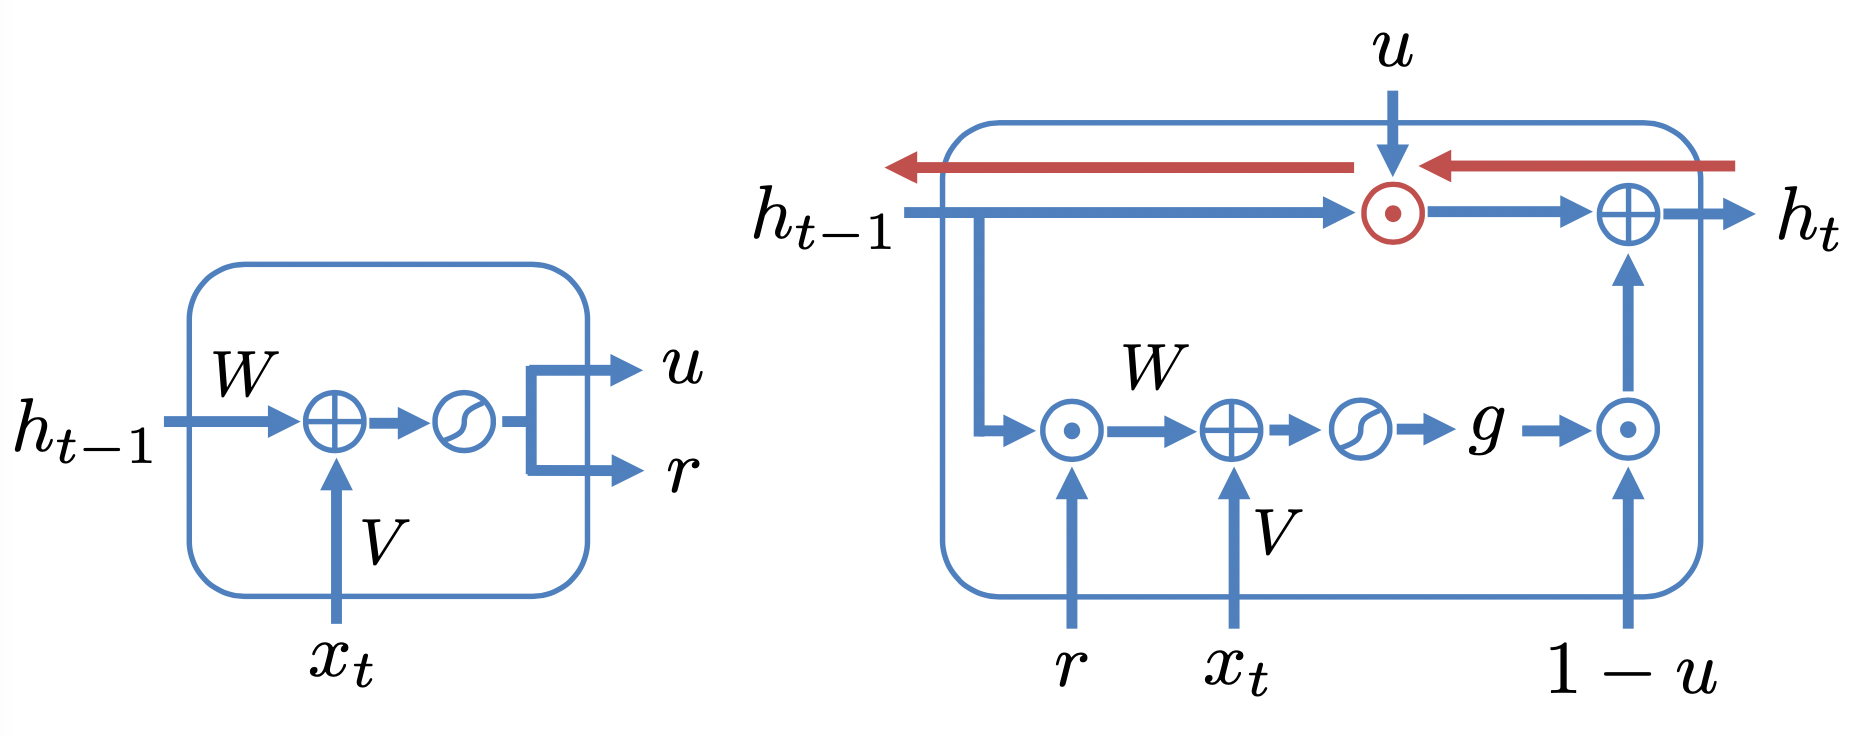
\includegraphics[scale=0.2]{gru.png} 
\end{center}

Пусть гейт $u$ оказался нулевым. Что это означает для нашей сетки? 
\begin{answerlist}
  \item Предыдущее скрытое состояние будет проигнорировано
  \item Значение $x_t$ никак не повлияет на прогноз $y_t$ 
  \item Текущее скрытое состояние никак не повлияет на формирование $g$
  \item Гейт $r$ окажется равен единице
  \item Кандидат в скрытое состояние не передаст на следующий шаг новой информации
\end{answerlist}
\end{question}

\begin{solution}
\begin{answerlist}
  \item Good answer :)
  \item Bad answer :(
  \item Bad answer :(
  \item Bad answer :(
  \item Bad answer :(
\end{answerlist}
\end{solution}



\begin{question}
Выберите все верные утверждения про предобработку текстов
\begin{answerlist}
  \item Очень часто встречающиеся слова (стоп-слова) обычно выкидывают из данных
  \item Сделать лемматизацию намного быстрее, чем стемминг 
  \item Очень редко встречающиеся слова обычно оставляют в данных
  \item Подсчёт idf занижает важность стоп-слов
  \item Подсчёт tf занижает важность стоп-слов
\end{answerlist}
\end{question}

\begin{solution}
\begin{answerlist}
  \item Good answer :)
  \item Bad answer :(
  \item Bad answer :(
  \item Good answer :)
  \item Bad answer :(
\end{answerlist}
\end{solution}





\begin{question}
Мы обучаем word2vec. В словаре $n$ слов. Мы учим вектора размерности $d$ с помощью skip-gram. Сколько параметров мы будем обучать в рамках такого подхода? 
\begin{answerlist}
  \item  $n$
  \item  $d$
  \item  $n \cdot d$
  \item  $2 \cdot n \cdot d$
  \item  $n \cdot d + 1$
\end{answerlist}
\end{question}

\begin{solution}
\begin{answerlist}
  \item Bad answer :(
  \item Good answer :)
  \item Bad answer :(
  \item Good answer :)
  \item Bad answer :(
\end{answerlist}
\end{solution}


\begin{question}
Одно из слабых мест классического механизма внимания -- время его работы. На вход в трансформер приходит текст длины $n$. Какова сложность по времени работы механизма self-attention? 
\begin{answerlist}
  \item $O(n)$
  \item $O(n^2)$
  \item $O(n^3)$
  \item $O(2^n)$
  \item $O(n!)$
\end{answerlist}
\end{question}

\begin{solution}
\begin{answerlist}
  \item Bad answer :(
  \item Good answer :)
  \item Bad answer :(
  \item Bad answer :(
  \item Bad answer :(
\end{answerlist}
\end{solution}

\newpage

\begin{question}
Выберите все верные утверждения про трансформеры
\begin{answerlist}
  \item Для каждого токена с помощью полносвязного слоя считаются три сущности: ключ (key), значение (value) и запрос (query)
  \item Внутри каждого слоя энкодера есть остаточная связь (residual connection)
  \item Обучение трансформера можно распаралелить, именно для этого его делают многоголовым (multihead self-attention)
  \item Внутри трансформера также как и в RNN используются рекуррентные ячейки
  \item В декодере кроме механизма самовнимания (self-attention) есть ещё и механизм внимания, на вход в который идёт выход энкодера
\end{answerlist}
\end{question}

\begin{solution}
\begin{answerlist}
  \item Bad answer :(
  \item Good answer :)
  \item Bad answer :(
  \item Good answer :)
  \item Bad answer :(
\end{answerlist}
\end{solution}


\begin{question}
    Представим, что у вас есть генеративная нейронная сеть (GAN), которая генерирует картинки с яблоками. Какое утверждение из представленных ниже неверное:
    \begin{answerlist}
      \item Основная цель генератора --- выучить распределение картинок с яблоками.
      \item После того, как мы обучим GAN, мы можем использовать дискриминатор, чтобы отличать яблоки от ананасов. 
      \item После обучения GAN ошибка дискриминатора стабилизируются около какой-то константы. 
      \item Генератор может создавать изображения с яблоками, которых никогда не существовало в природе. 
      \item Генератор и Дискриминатор нужно обучать последоввательно. Сначала несколько шагов обучения генератора, потом дискриминатора.
    \end{answerlist}
\end{question}

\begin{solution}
\begin{answerlist}
  \item Bad answer :(
  \item Good answer :)
  \item Bad answer :(
  \item Good answer :)
  \item Bad answer :(
\end{answerlist}
\end{solution}



\begin{question}
Думал(а) когда-нибудь о том, чтобы сбежать из дома и жить в пещере?
\begin{answerlist}
  \item Да, ведь я сторонник анархо-примитивизма
  \item Только если роботы захватят мир
  \item Да, обожаю ходить по дому голым, в пещере никто не сможет заставить меня одеться
  \item Нет, там холодно и сыро
  \item Да, потому что мама заставляет меня мыть посуду, а я больше не могу мыть посуду
\end{answerlist}
\end{question}

\begin{solution}
\begin{answerlist}
  \item Bad answer :(
  \item Good answer :)
  \item Bad answer :(
  \item Good answer :)
  \item Bad answer :(
\end{answerlist}
\end{solution}

\newpage 

\section*{Часть вторая: вопросы и задачки}

Все ответы должны быть обоснованы. Решения должны быть прописаны для каждого пункта. Рисунки должны быть чёткими и понятными. Все линии должны быть подписаны. За решение каждой задачи можно получить 8 баллов.

\begin{question}
    Илон Маск учит FastText для словаря из $n$ слов. Все слова состоят из букв латинского алфавита ($26$ букв). Другие символы в корпусе не встречаются. Сколько параметров нужно оценить Илону Маску? Как можно будет применить модель к новым словам, которых не было в словаре?
\end{question}

\vspace{8cm} 

\begin{question}
    Выпишите уравнения, описывающие LSTM-ячейку с забыванием и GRU-ячейку. Какие после- довательности и веса нужно занулить, чтобы эти ячейки превратились в простую RNN-ячейку?
\end{question}

\newpage

 
\begin{question}
Объясните в чём заключается смысл механизма self-attention в трансформерах. Выпишите основные формулы. 
\end{question}

\vspace{8cm} 

\begin{question}
Объясните в чём заключается главный недостаток Greedy Decoding. Как Beam Search пытается решить этот недостаток? 
\end{question}

\newpage

\begin{question}
Объясните чем GPT отличается от BERT. Как это все связано с архитектурой трансформера? Почему в расшифровке BERT (Bidirectional Encoder Representations from Transformers) встречается слово Bidirectional? 
\end{question}

\vspace{8cm} 


\begin{question}
Предположим, что вы обучили два w2v на разных корпусах текстов. Как бы вы выяснили, у какой из моделей более хорошее качество? 
\end{question}



\newpage 

\section*{Часть третья: ML-design}

За эту задачу вы можете получить максимально 20 баллов. Попробуйте как можно чётче структурировать свои мысли. Опишите какие данные вам 


\begin{question}
Когда пользователь в поисковике печатает свой запрос, под строкой ввода ему обычно показываются разные варианты продолжения его запроса и другие варианты запроса (саджесты).  

\begin{center} 
    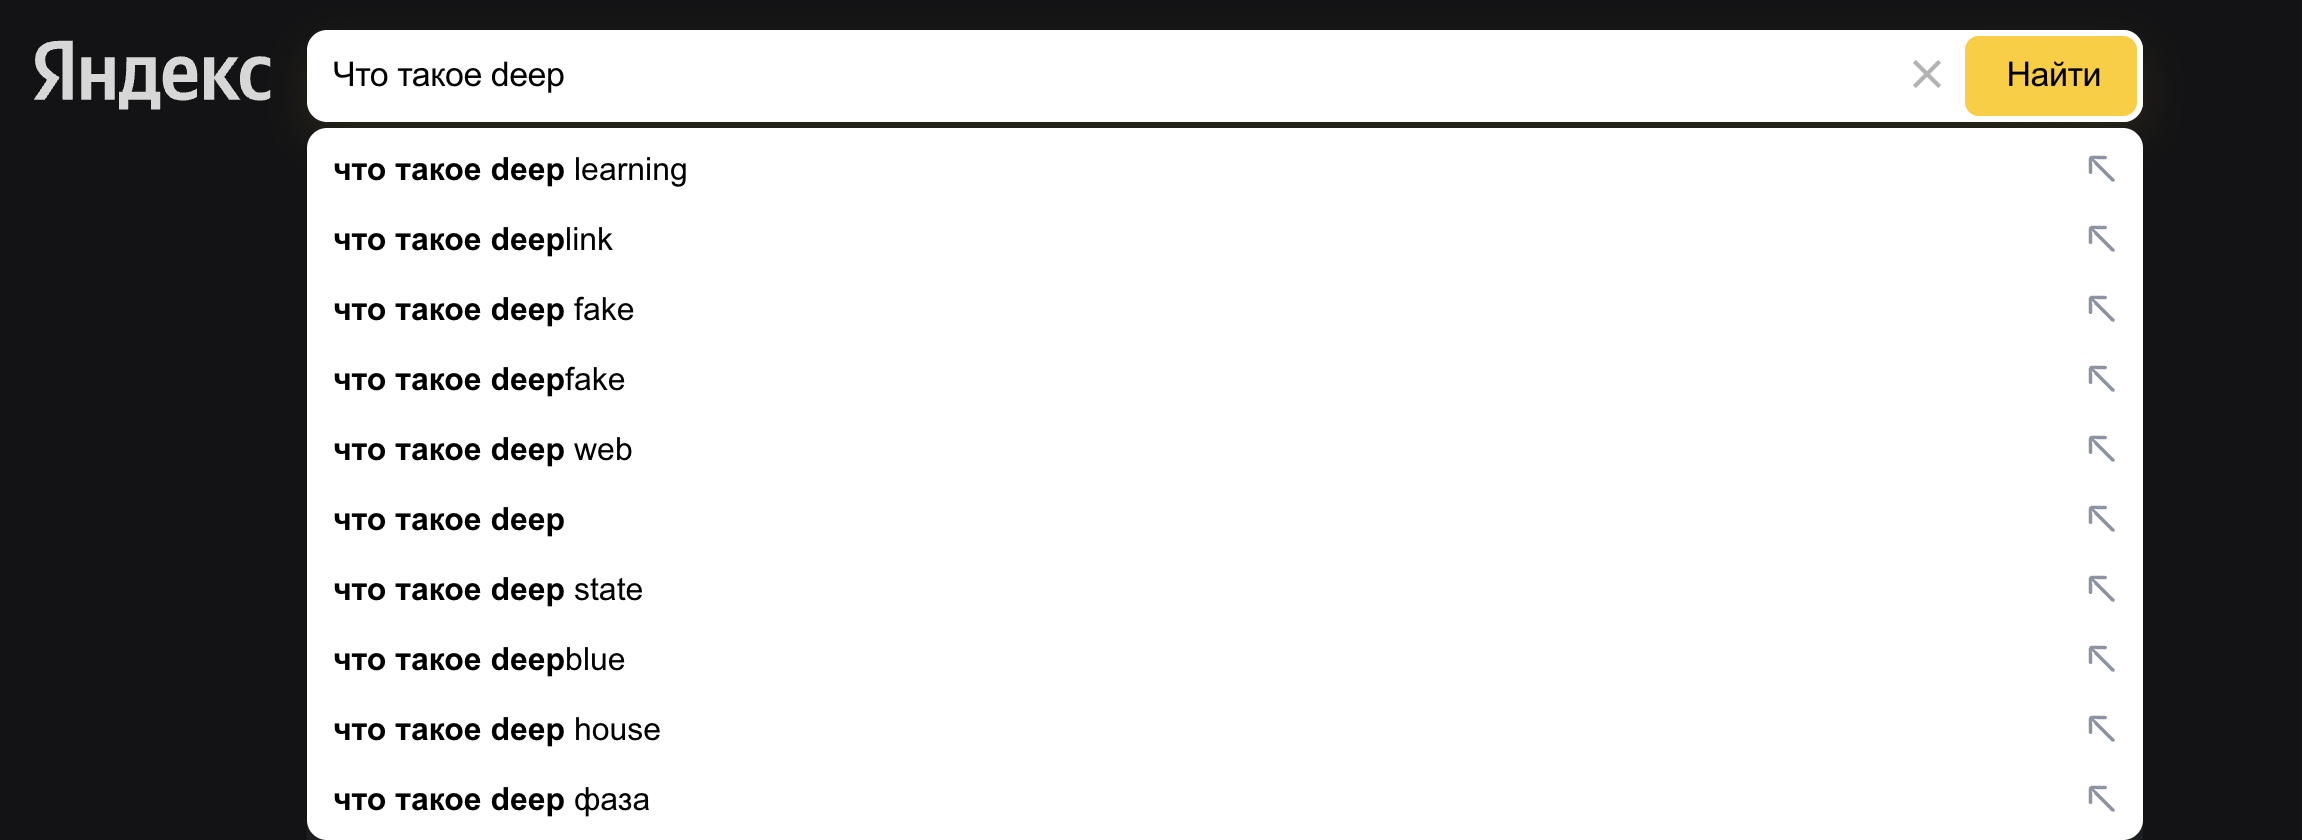
\includegraphics[scale=0.45]{sudjest.png} 
\end{center}

Вы устроились в крупную технологическую компанию ML-инженером и вам нужно реализовать такой механизм. Как бы вы решали такую задачу? 

\begin{itemize} 
    \item Как бы вы сформулировали задачу ML? 
    \item Как бы вы собирали выборку, факторы, разметку? 
    \item Как бы вы сформулировали таргет? 
    \item Что бы вы использовали в качестве бейзлайна (изначальное очень простое решение)? 
    \item Какую модель вы бы использовали? Как бы вы её обучали? 
    \item Как бы вы проверили качество внедрения? 
\end{itemize} 
\end{question}


\end{document}
